\documentclass[letterpaper,10pt]{article}
\usepackage[pdftex]{graphicx}
\usepackage{listings}
\usepackage{alltt}
\usepackage{color}
\usepackage{amsmath}
\usepackage{hyperref}
\usepackage{pgfplotstable}

\definecolor{dkgreen}{rgb}{0,0.6,0}
\definecolor{gray}{rgb}{0.5,0.5,0.5}
\definecolor{mauve}{rgb}{0.58,0,0.82}

\hypersetup{
    colorlinks,
    citecolor=black,
    filecolor=black,
    linkcolor=black,
    urlcolor=black
}

\lstset{
	basicstyle=\footnotesize,
	breaklines=true,
	 backgroundcolor=\color{white},   % choose the background color; you must add \usepackage{color} or \usepackage{xcolor}
  basicstyle=\footnotesize,        % the size of the fonts that are used for the code
  breakatwhitespace=false,         % sets if automatic breaks should only happen at whitespace
  breaklines=true,                 % sets automatic line breaking
  captionpos=b,                    % sets the caption-position to bottom
  commentstyle=\color{dkgreen},    % comment style
  deletekeywords={...},            % if you want to delete keywords from the given language
  escapeinside={\%*}{*)},          % if you want to add LaTeX within your code
  extendedchars=true,              % lets you use non-ASCII characters; for 8-bits encodings only, does not work with UTF-8
  frame=single,	                   % adds a frame around the code
  keepspaces=true,                 % keeps spaces in text, useful for keeping indentation of code (possibly needs columns=flexible)
  keywordstyle=\color{blue},       % keyword style
  otherkeywords={*,grep,sort,head,mv,perl,chmod,...},           % if you want to add more keywords to the set
  numbers=left,                    % where to put the line-numbers; possible values are (none, left, right)
  numbersep=5pt,                   % how far the line-numbers are from the code
  numberstyle=\tiny\color{gray}, % the style that is used for the line-numbers
  rulecolor=\color{black},         % if not set, the frame-color may be changed on line-breaks within not-black text (e.g. comments (green here))
  showspaces=false,                % show spaces everywhere adding particular underscores; it overrides 'showstringspaces'
  showstringspaces=false,          % underline spaces within strings only
  showtabs=false,                  % show tabs within strings adding particular underscores
  stepnumber=1,                    % the step between two line-numbers. If it's 1, each line will be numbered
  stringstyle=\color{mauve},     % string literal style
  tabsize=2,	                   % sets default tabsize to 2 spaces
  title=\lstname                   % show the filename of files included with \lstinputlisting; also try caption instead of title
}


\begin{document} 

\begin{titlepage}

\begin{center}

\Huge{Assignment 4}

\Large{CS532-s16:  Web Sciences}

\Large{Spring 2016}

\Large{John Berlin}

\Large Generated on \today

\end{center}

\end{titlepage}
\newpage
\section*{1}
\subsection*{Question}
\begin{verbatim}
1.  Determine if the friendship paradox holds for my Facebook
account.* Compute the mean, standard deviation, and median of the
number of friends that my friends have.  Create a graph of the
number of friends (y-axis) and the friends themselves, sorted by
number of friends (x-axis).  (The friends don't need to be labeled
on the x-axis: just f1, f2, f3, ... fn.)  Do include me in the graph
and label me accordingly.

* = This used to be more interesting when you could more easily download
your friend's friends data from Facebook.  Facebook now requires each
friend to approve this operation, effectively making it impossible.

I will email to the list the XML file that contains my Facebook
friendship graph ca. Oct, 2013.  The interesting part of the file looks
like this (for 1 friend):

<node id="Johan_Bollen_1448621116">
        <data key="Label">Johan Bollen</data>
        <data key="uid"><![CDATA[1448621116]]></data>
        <data key="name"><![CDATA[Johan Bollen]]></data>
        <data key="mutual_friend_count"><![CDATA[37]]></data>
        <data key="friend_count"><![CDATA[420]]></data>
</node>

It is in GraphML format: http://graphml.graphdrawing.org/
\end{verbatim}
\subsection*{Answer}
After downloading the \verb+GraphML+ file and visually inspecting it I thought to myself there has to be a library for this. As usual there was one for python called \emph{Pygraphml} \cite{pygraphml}. Using this library made parsing and extraction of the information easy. The python script to extract the information is found in listing \ref{lst:pgraph}. The process was so easy please as the library puts all data portions of a node inside of a dictionary and simply loop through the nodes of the graph for them.

As usual be sure to be in the directory containing the graphml file. 
To run the script execute it as such:
\begin{lstlisting}[frame=single]
$ chmod +x parseGraph.py
$ ./parseGraph.py
\end{lstlisting}

After the Python script finishes running it will produce a file called \emph{mlnfbcount.csv}. This file contains the number of friends Dr. Nelson's friends have as well as an entry of how many friends he has. His entry is not included in the calculations of the mean, median, and standard deviation. Those calculations can be found in table \ref{stats:fb}. 
\begin{table}
\centering
\begin{tabular}{ l l }
\textbf{Mean} & 358.987 \\
\textbf{Median} & 266.5 \\
\textbf{Std Dev} &  371.585 \\
\end{tabular}
\caption{Statistics from MLN Facebook friends}
\label{stats:fb}
\end{table}



Dr. Nelson has \verb+154+ Facebook friends which means he has less friends than his Facebook friends. How can I be sure of that. For one he has less friends than the median. Secondly I used the R script found in listing \ref{lst:fbpr}  to generate the plot seen in figure \ref{fig:fbp} to calculate what percent of his friends have more or less friends than him. Those results are seen below.
\begin{lstlisting}[frame=single]
mln has less fb friends than  72.26% of his friends
mln has more fb friends than  27.1% of his friends
\end{lstlisting}


Since the calculation done in R even say that Dr. Nelson has less friends than 72.26 percent of his own friends the paradox holds.


\newpage
\lstinputlisting[language=Python,frame=single,
caption={Parse and Extract Dr. Nelson Facebook graph},label=lst:pgraph,captionpos=b]{parseGraph.py}

\newpage
\begin{figure}[h]
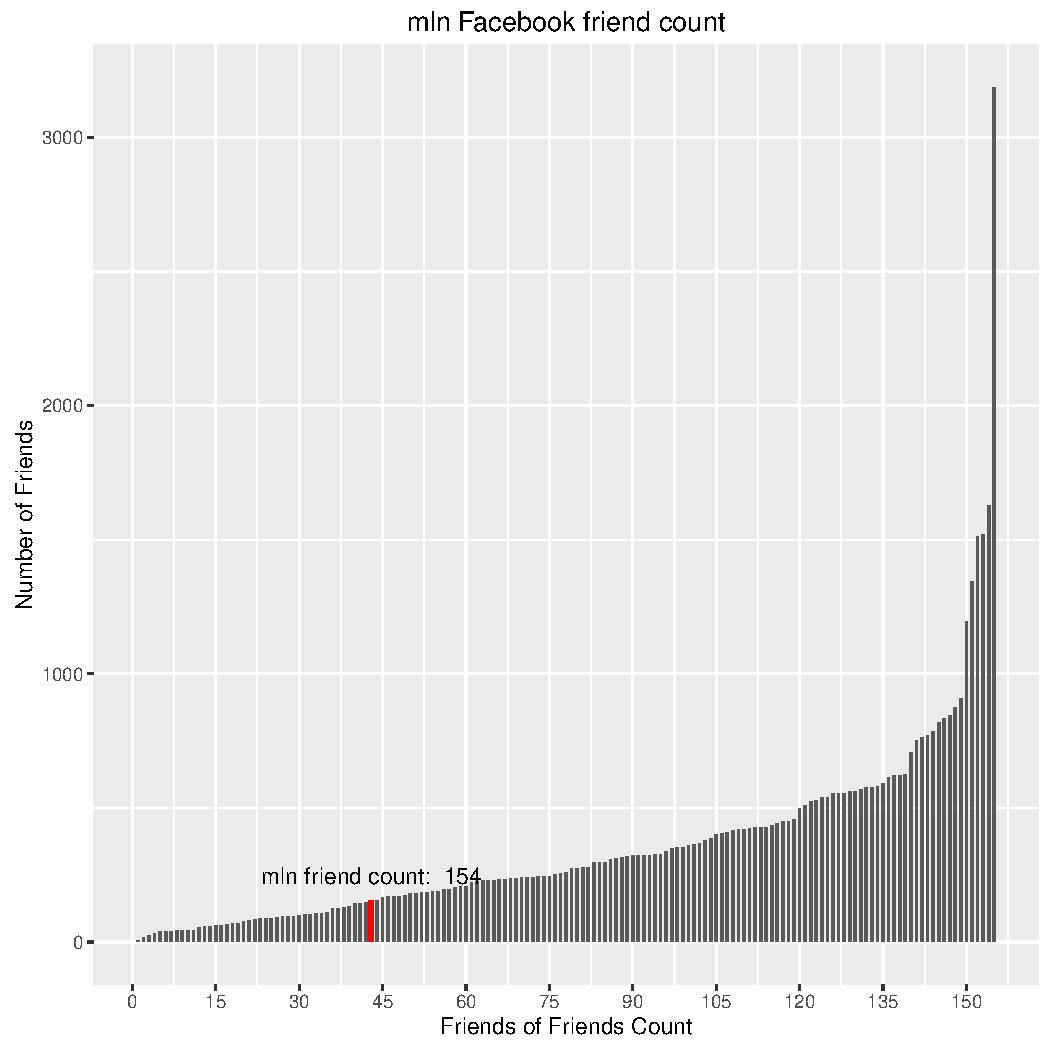
\includegraphics[scale=0.7]{mlnFacebookParadox.pdf}
\caption{Bar plot showing the count of Dr. Nelson's Facebook Friends' Friends}
\label{fig:fbp}
\end{figure}
\newpage
\lstinputlisting[language=R,frame=single,caption={R script to generate \ref{fig:fbp}},label=lst:fbpr,captionpos=b,numbers=left,showspaces=false,showstringspaces=false,basicstyle=\footnotesize]{mlnFriendParadox.R} 
 \newpage
\section*{2}
\subsection*{Question}
\begin{verbatim}
 2.  Determine if the friendship paradox holds for your Twitter account.
Since Twitter is a directed graph, use "followers" as value you measure
(i.e., "do your followers have more followers than you?").

Generate the same graph as in question #1, and calcuate the same 
mean, standard deviation, and median values.

For the Twitter 1.1 API to help gather this data, see:

https://dev.twitter.com/docs/api/1.1/get/followers/list

If you do not have followers on Twitter (or don't have more than 50),
then use my twitter account "phonedude_mln".
\end{verbatim}
\subsection*{Answer}

As I do not have the required amount of twitter followers, I resorted to using Dr. Nelson's Twitter followers to answer this question. The python script in listing \ref{lst:ptwittter} contains both the code used to generate the number of followers \verb+@phonedude_mln+ followers have as well as the followers the people he is following.  

To run the script execute it as such:
\begin{lstlisting}[frame=single]
$ chmod +x getTwitterFollowers.py
$ ./getTwitterFollowers.py
\end{lstlisting}

The python script uses the \emph{Tweepy} library to abstract the communication with the \emph{Twitter} api. The process of getting this information in brief is as such. 
\begin{enumerate}
\item Set up OAuth. I left out my keys and can easily be replaced with your own by using a config.py file
\item Get an instance of the API
\item Execute methods mlnfollowing and mlnfollowers. Both methods execute as such
\begin{enumerate}
\item Open a cursor to query the Twitter api for friends or followers
\item Get the response and add it to a list
\item After all items have been gotten extract the friend or followers name and followers count
\item Write results to a file
\end{enumerate}
\end{enumerate}

After consulting the output it was found \verb+@phonedude_mln+ has 489 followers.  
The R script seen in listing \ref{lst:tw1pr} was used to generate the graph in figure \ref{fig:twfp} and the stats seen in table \ref{stats:twfst}. For more details on the process of the R script \ref{lst:tw1pr} please consult the comments. 
\begin{table}
\centering
\begin{tabular}{ l l }
\textbf{Mean} & 1047.01 \\
\textbf{Median} & 258 \\
\textbf{Std Dev} &  4150.377 \\
\end{tabular}
\caption{Statistics for @phonedude\_mln Twitter Followers}
\label{stats:twfst}
\end{table}

Since \verb+@phonedude_mln+ has 489 and is shown in the plot in figure \ref{fig:twfp} he does not have more followers than his followers.  As seen below in the output from running the R script seen in listing \ref{lst:tw1pr} Dr. Nelson has 63.67 percent more followers than his followers. 

\begin{lstlisting}[frame=single]
phonedude_mln has less twitter followers than  36.12 % of his followers
phonedude_mln has more twitter followers than  63.67 % of his followers
\end{lstlisting}

From this it is clear to see that the friendship paradox does not hold here.

Please note that the figure generated to answer this question has the y-axis in log10 scale.
\newpage
\begin{figure}
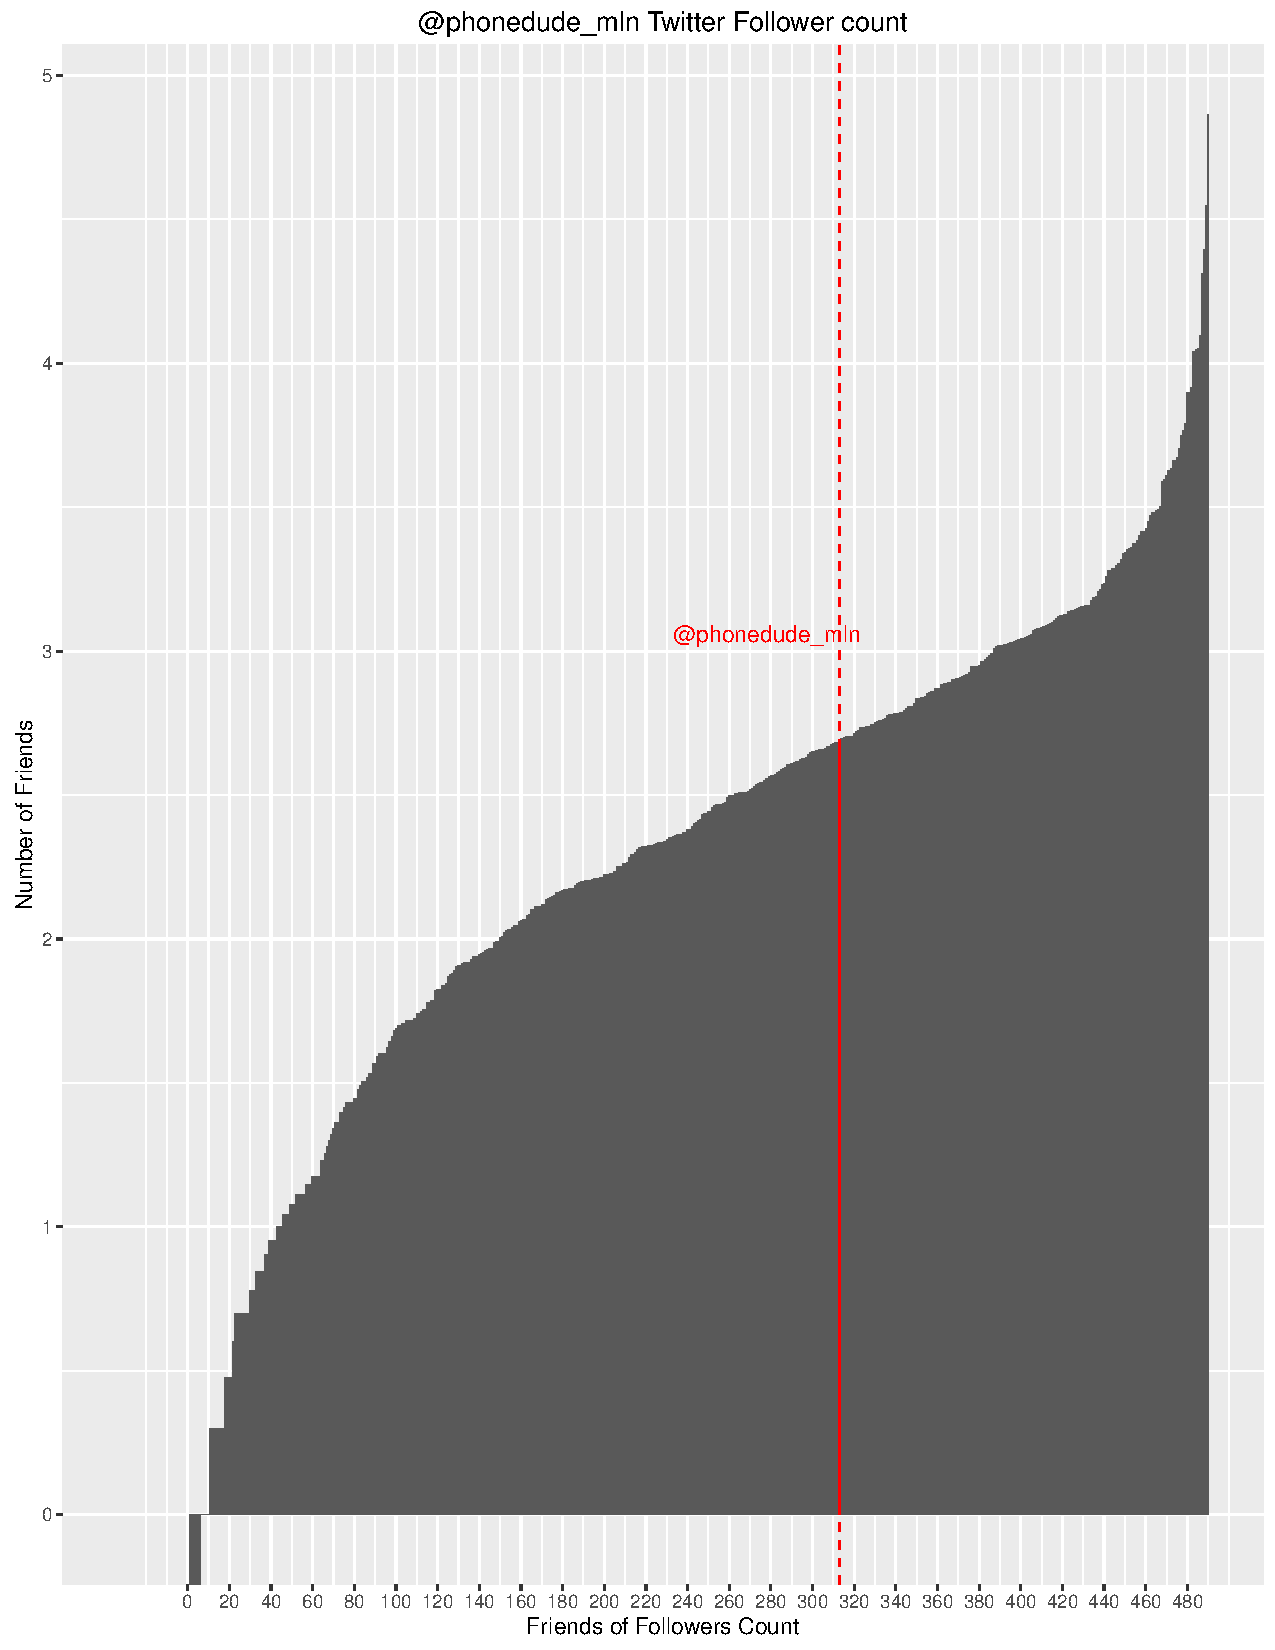
\includegraphics[scale=0.6]{mlnTwitterFollowerParadox.pdf}
\caption{Bar plot showing the count of Dr. Nelson's Twitter Followers Friends}
\label{fig:twfp}
\end{figure}
\newpage
\lstinputlisting[language=Python,frame=single,
caption={Parse and Extract Dr. Nelson Facebook graph},label=lst:ptwittter,captionpos=b]{getTwitterFollowers.py}



 
\lstinputlisting[language=R,frame=single,caption={R script to generate \ref{fig:twfp}},label=lst:tw1pr,captionpos=b,numbers=left,showspaces=false,showstringspaces=false,basicstyle=\footnotesize]{mlnTwitterFollower.R} 

\newpage
 
\section*{3}

\subsection*{Question}

\begin{verbatim}
Extra credit, 2 points:

3.  Repeat question #1, but with your LinkedIn profile.
\end{verbatim}
\subsection*{Answer}

Not attempted. As I was unable to nicely get the LinkedIn api to generate keys.

\newpage
\section*{4}
\subsection*{Question}
\begin{verbatim}
Extra credit, 1 point:

4.  Repeat question #2, but change "followers" to "following"?  In
other words, are the people I am following following more people?
\end{verbatim}
\subsection*{Answer}
The same python script seen in listing \ref{lst:ptwittter} was used to generate this data. At the time when I got this data \verb+@phonedude_mln+ had 227 Friends or people he was personally following. 
The R script in listing \ref{lst:twitterfriend} is used to produce the stats seen in table \ref{stats:twfst2} and the resulting plot which is also in log10 scale seen in figure \ref{fig:twfp2}

Dr. Nelson has a mean number of followers for friends of 748 which is clearly greater than his own number friend at 227. The output from the R script stats:
\begin{lstlisting}[frame=single]
@phonedude_mln has less twitter friends than  70.61 % of his friends
@phonedude_mln has more twitter friends than  28.95 % of his friends
\end{lstlisting}

So \verb+@phonedude_mln+ has less twitter friends than 70.61 percent of his friends thus the paradox holds.

\begin{figure}[h]
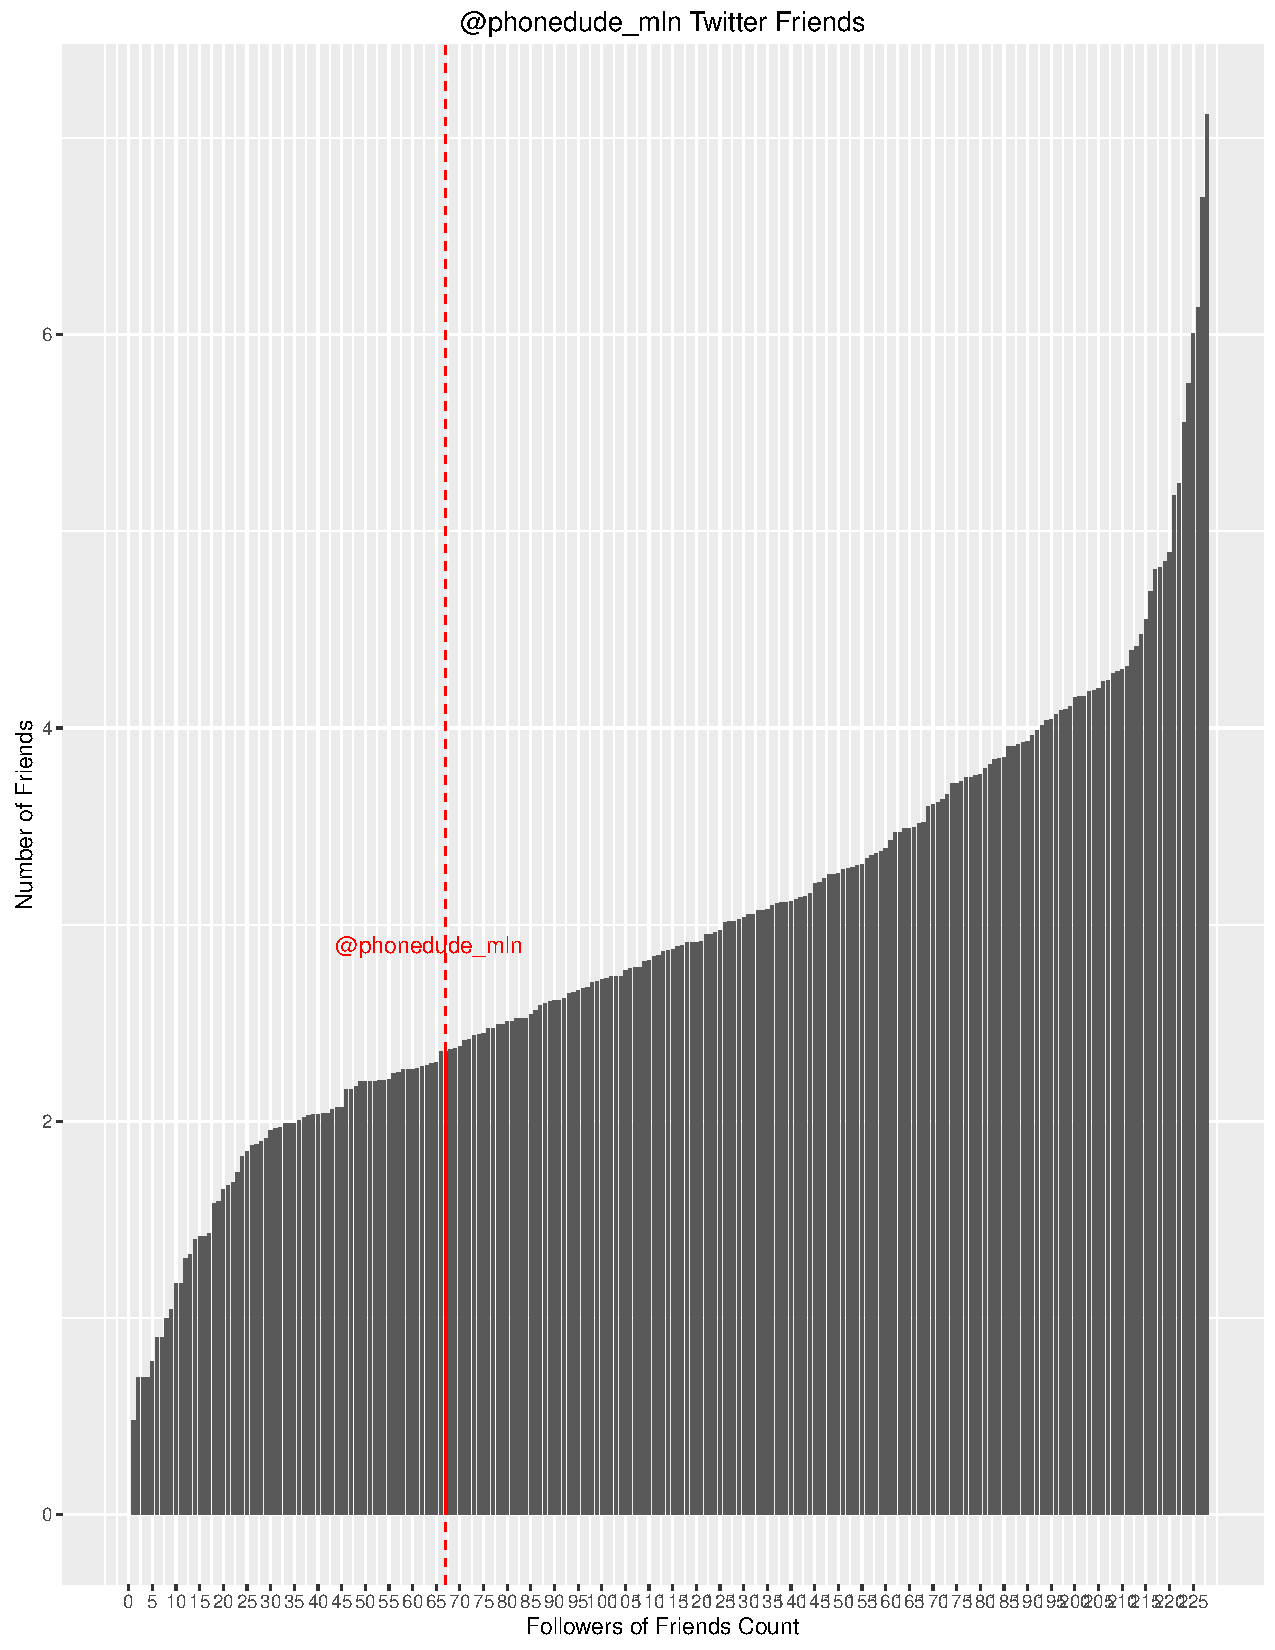
\includegraphics[scale=0.6]{mlnTwitterFriendParadox.pdf}
\caption{Bar plot showing the count of Dr. Nelson's Twitter Friends Friends}
\label{fig:twfp2}
\end{figure}
\begin{table}
\centering
\begin{tabular}{ l l }
\textbf{Mean} & 100257.974 \\
\textbf{Median} & 748 \\
\textbf{Std Dev} &  937488.014 \\
\end{tabular}
\caption{Statistics for @phonedude\_mln Twitter F}
\label{stats:twfst2}
\end{table}
 \newpage
 
\lstinputlisting[language=R,frame=single,caption={R script to calculate the Friendship Paradox for Twitter Friends},label=lst:twitterfriend,captionpos=b,numbers=left,showspaces=false,showstringspaces=false,basicstyle=\footnotesize]{mlnTwitterFriend.R} 
\newpage
\clearpage
\bibliographystyle{acm}
\bibliography{references}        
\end{document}